\documentclass[letterpaper,oneside]{book}
\usepackage[letterpaper,left=1in,right=1in,top=1in,bottom=1in]{geometry}
\usepackage{setspace,epsfig,subfigure,rawfonts,graphicx,graphicx,epsf,psfrag}
\usepackage{amssymb,amsfonts,amsmath,amsthm}
\usepackage[noadjust]{cite}
\usepackage{appendix}
\usepackage{array}
\usepackage{eqparbox}
\usepackage{multirow}
\usepackage{chngcntr}
\usepackage{etoolbox}
\usepackage[chapter]{algorithm}
\usepackage{algorithmic}
\usepackage{bm}
\usepackage{titlesec}
\usepackage{lipsum}
\usepackage[nottoc,notlot,notlof]{tocbibind}
\usepackage{physics}


\renewcommand{\bibname}{References}

\AtBeginEnvironment{subappendices}{%
\chapter*{Appendix}
\addcontentsline{toc}{chapter}{Appendices}
\counterwithin{figure}{chapter}
\counterwithin{table}{chapter}
}

\titleformat{\chapter}[display]
{\normalfont\LARGE\bf}
{\chaptertitlename\ \thechapter}{15pt}{}
  
\titlespacing*{\chapter}{0pt}{-20pt}{40pt}

\newcounter{exercisectr}
\newenvironment{exercise}[1][]{%      define a custom environment
   \medskip\noindent%         create a vertical offset to previous material
   \refstepcounter{exercisectr}% increment the environment's counter
   \large{\textbf{Ex. \theexercisectr\ #1}}% or \textbf, \textit, ...
   \newline%
   }{\par\medskip}  %          create a vertical offset to following material
\numberwithin{exercisectr}{chapter}

\begin{document}

\doublespacing
\renewcommand{\labelenumi}{(\arabic{enumi})}

\title{
  {\huge A Partial Solution Manual for: \emph{The Elements of Statistical
  Learning} by Jerome Friedman, Trevor Hastie, and Robert Tibshirani}
}

\author{
  Wenhao Wu\\
  wnhwu@ucdavis.edu\\
  Dept. ECE, UC Davis\\
}
\date{\today}
\maketitle

\onehalfspacing
\pagenumbering{roman}
\tableofcontents

%\newpage
\pagenumbering{arabic}
%\newpage
\chapter*{Preface}
\addcontentsline{toc}{chapter}{Preface}

This work is expected to be used as a supplementary material for Weatherwax and
Epstein's solution manual~\cite{weatherwax2013solution}, which I found to be
very helpful when self-studying this popular textbook. The numbering of chapters
and problems are based on the 2nd edition (10th printing with corrections, Jan 2013) available
online~\cite{friedman2009elements}.

The author was not able to solve all the excercises. Even for the solutions
included we expect many mistakes and shortcomings. It would be of great help if
people could suggest possible solutions or help us find and correct the errors
so this solution manual can be continuously improved to benefit more interested
readers. We are also open to all comments and criticisms. Our contact
information can be found at the website holding this draft~\cite{wu2016partial}.


\chapter*{Acknowledgment}
\addcontentsline{toc}{chapter}{Acknowledgment}

\setcounter{chapter}{1}
\chapter{Overview of Supervised Learning}
\label{ch:2} % Chapter 2
\chapter{Linear Methods for Regression}
\label{ch:3} % Chapter 3
\chapter{Linear Methods for Classification}
\label{ch:4} % Chapter 4
\chapter{Basis Expansions and Regularization}
\label{ch:5} % Chapter 5
\chapter{Kernel Smoothing Methods}
\label{ch:6} % Chapter 6
\chapter{Model Assessment and Selection}
\label{ch:7} % Chapter 7
\chapter{Model Inference and Averaging}
\label{ch:8} % Chapter 8
\chapter{Additive Models, Trees, and Related Methods}
\label{ch:9} % Chapter 9
\chapter{Boosting and Additive Trees}
\label{ch:10}

\begin{exercise}
  To minimize the exponential loss function (defined between Eq. (10.10) and
  (10.11))
  \begin{align}
    L_m(\beta) &= \sum_{i=1}^Nw_i^{(m)}\exp(-\beta y_iG_m(x_i)) \notag\\
    &= \exp(-\beta)\sum_{y_i=G_m(x_i)}w_i{(m)} +
    \exp(\beta)\sum_{y_i\not=G_m(x_i)}w_i{(m)}
  \end{align}
  the stationary condition suggests that
  \begin{align}
    \pdv{L_m}{\beta} &= -\exp(-\beta)\sum_{y_i=G_m(x_i)}w_i{(m)} +
    \exp(\beta)\sum_{y_i\not=G_m(x_i)}w_i{(m)}=0
  \end{align}
  therefore
  \begin{align}
    \beta_m &= \frac{1}{2}\log\frac{\sum_{y_i=G_m(x_i)}w_i{(m)}}
    {\sum_{y_i\not=G_m(x_i)}w_i{(m)} } =
    \frac{1}{2}\log\frac{1-\overline{\mbox{err}}_m} {\overline{\mbox{err}}_m}
  \end{align}
\end{exercise}

\begin{exercise}
  \begin{align}
    \mathbb{E}_{Y|x} \left(e^{-Yf(x)}\right) = \mbox{Pr}(Y=1|x)e^{-f(x)} +
    \mbox{Pr}(Y=-1|x)e^{f(x)}
  \end{align}
  To minimize the loss function, we have
  \begin{align}
    \pdv{E}{f} &= -\mbox{Pr}(Y=1|x)e^{-f(x)} +
    \mbox{Pr}(Y=-1|x)e^{f(x)} = 0
  \end{align}
  therefore
  \begin{align}
    f^*(x) = \frac{1}{2}\log\frac{\mbox{Pr}(Y=1|x)}{\mbox{Pr}(Y=-1|x)}
  \end{align}
\end{exercise}

\begin{exercise}
  For Eq. (10.47), we have
  \begin{subequations}
    \begin{align}
      \mathbb{E}_{X_{\mathcal{C}}}[h_1(X_{\mathcal{S}}) + h_2(X_{\mathcal{C}})]
      & = h_1(X_{\mathcal{S}}) +
      \mathbb{E}_{X_{\mathcal{C}}}[h_2(X_{\mathcal{C}})]
      \\
      \mathbb{E}_{X_{\mathcal{C}}}[h_1(X_{\mathcal{S}}) h_2(X_{\mathcal{C}})]
      & = h_1(X_{\mathcal{S}})
      \mathbb{E}_{X_{\mathcal{C}}}[h_2(X_{\mathcal{C}})]
    \end{align}
  \end{subequations}
  since $\mathbb{E}_{X_{\mathcal{C}}}[h_2(X_{\mathcal{C}})]$ is a constant
  independent of $X_{\mathcal{S}}$, the marginal average recovers additive and
  multiplicative functions. On the other hand,
  \begin{subequations}
    \begin{align}
      \mathbb{E}_{X_{\mathcal{C}}|X_{\mathcal{S}}}[h_1(X_{\mathcal{S}}) +
      h_2(X_{\mathcal{C}})] & = h_1(X_{\mathcal{S}}) +
      \mathbb{E}_{X_{\mathcal{C}}|X_{\mathcal{S}}}[h_2(X_{\mathcal{C}})]
      \\
      \mathbb{E}_{X_{\mathcal{C}}|X_{\mathcal{S}}}[h_1(X_{\mathcal{S}})
      h_2(X_{\mathcal{C}})] & = h_1(X_{\mathcal{S}})
      \mathbb{E}_{X_{\mathcal{C}}|X_{\mathcal{S}}}[h_2(X_{\mathcal{C}})]
    \end{align}
  \end{subequations}
  unless $X_{\mathcal{C}}$ and $X_{\mathcal{S}}$ are independent, $
  \mathbb{E}_{X_{\mathcal{C}}|X_{\mathcal{S}}}[h_2(X_{\mathcal{C}})]$ is a
  function of the value of $X_{\mathcal{S}}$.
\end{exercise}

\begin{exercise}[(Program)]
\end{exercise}

\begin{exercise}
  \begin{exerciseSection}
    Since $\sum_{k=1}^Kf_k =0$,
    \begin{align}
      E(Y,f) &= \mathbb{E}_{Y|x}\left[\exp\left(-\frac{1}{K}\sum_{k=1}^Kf_kY_k
       \right) \right] \notag\\
       &= \sum_{k=1}^K P_{G|x}(G=\mathcal{G}_k|x) \exp\left(-\frac{1}{K}f_k +
       -\frac{1}{K(K-1)}\sum_{j\not=k}f_j \right) \notag\\
       &= \sum_{k=1}^K P_{G|x}(G=\mathcal{G}_k|x) \exp\left(-\frac{1}{K-1}f_k \right)
    \end{align}
    Denote the Lagrangian as $l(f, \lambda) =  E(Y,f) +
    \lambda(\sum_{k=1}^Kf_k - 1)$. To minimize $E(Y,f)$, we have
    \begin{align}
      \pdv{l}{f_k} = P_{G|x}(G=\mathcal{G}_k|x) \exp\left(-\frac{1}{K-1}f_k
      \right)\left(-\frac{1}{K-1}\right) + \lambda = 0
    \end{align} 
    therefore
    \begin{align}
      f_k(x) = -(K-1)\log\frac{(K-1)\lambda}{P_{G|x}(G=\mathcal{G}_k|x)}
    \end{align}
    $\lambda$ can be by substituting the above equation into $\sum_{k=1}^Kf_k
    =0$, which leads to
    \begin{align}
      \log[(K-1)\lambda] = \frac{1}{K}\sum_{k=1}^K\log
      P_{G|x}(G=\mathcal{G}_k|x)
    \end{align}
    Consequently,
    \begin{align}
      f_k(x) &= (K-1)\left[\log P_{G|x}(G=\mathcal{G}_k|x) -
      \frac{1}{K}\sum_{j=1}^K \log P_{G|x}(G=\mathcal{G}_j|x) \right].
    \end{align}
    Note that the first term in the squared bracket is the log-likelihood of
    $x$ belonging to class $k$, while the second term is the mean-log-likelihood
    of $x$ among all the $K$ classes.
  \end{exerciseSection}
  \begin{exerciseSection}
    (Here $\beta_m$ is a scalar, $f_m, G_m$ are $K$-by-1 vectors and $y_i$ is a
    1-by-$K$ vector.) We derive the multiclass boosting algorithm following
    a similar process starting from Eq. (10.9):
    \begin{align}
      (\beta_m, G_m) = \arg\min_{\beta, G}\sum_{i=1}^Nw_i^{(m)}\exp(-\beta
      y_iG(x_i))
    \end{align}
    where $w_i^{(m)} = \exp(-y_if_{m-1}(x_i))$, and $G$ is the output of a
    $K$-class classifier encoded exactly the same way as $Y$.
    Again we solve this problem in two steps. To solve $G_m$, the exponential
    loss function can be rewritten as
    \begin{align}
      L^{(m)}(\beta, G) &= \sum_{i=1}^Nw_i^{(m)} \exp(-\beta
      y_iG(x_i)) \notag\\
      &= \sum_{y_i=G(x_i)}w_i^{(m)}\exp\left(-\beta\left[1 +
      \frac{1}{K-1}\right]\right) \notag\\ 
      &+
      \sum_{y_i\not=G(x_i)} w_i^{(m)}\exp\left(-\beta\left[-\frac{2}{K-1} +
      \frac{K-2}{(K-1)^2}\right]\right) \notag\\
      &= \sum_{y_i=G(x_i)}w_i^{(m)}\exp\left(-
      \frac{K}{K-1}\beta\right) +
      \sum_{y_i\not=G(x_i)} w_i^{(m)}\exp\left(\frac{K}{K-1}\beta\right)
      \notag\\
      &= \exp\left(-\frac{K}{K-1}\beta\right)\sum_{i=1}^Nw_i^{(m)} \notag\\
      &+ \left[\exp\left(\frac{K}{K-1}\beta\right) -
      \exp\left(-\frac{K}{K-1}\beta\right) \right]\sum_{i=1}^N w_i^{(m)}I(y_i\not=G(x_i))
    \end{align}
    therefore
    \begin{align}
      G_m = \arg\min_{G} \sum_{i=1}^Nw_i^{(m)} I(y_i\not=G(x_i))
    \end{align}
    which is exactly the same as Eq. (10.10).
    
    To solve $\beta_m$, we have
    \begin{align}
      \pdv{L^{(m)}(\beta, G)}{\beta} &=
      \frac{K}{K-1}\left[-\sum_{y_i=G(x_i)}w_i^{(m)}\exp\left(-\frac{K}{K-1}\beta\right)
      + \sum_{y_i\not=G(x_i)} w_i^{(m)}\exp\left(\frac{K}{K-1}\beta\right)\right] \notag\\
      &= 0
    \end{align}
    therefore
    \begin{align}
      \beta_m = \frac{K-1}{2K}\log\frac{\sum_{y_i=G(x_i)}w_i^{(m)}}
      {\sum_{y_i\not=G(x_i)}w_i^{(m)}} = \frac{K-1}{2K}
      \log\frac{1-\overline{\mbox{err}}_m} {\overline{\mbox{err}}_m}
    \end{align}
    for which Eq. (10.12) is a special case when $K=2$. In conclusion, the
    overall process is almost the same as Algorithm 10.1.
  \end{exerciseSection}
\end{exercise}

\begin{exercise}[(Program)]
\end{exercise}

\begin{exercise}
  Denote the loss function for region $R_{jm}$ to minimize in Eq.
  (10.30) as
  \begin{align}
    L_{jm} & = \sum_{x_i\in R_{jm}}w_i^{(m)}\exp(-y_i\gamma_{jm})\notag\\
    &= \sum_{x_i\in R_{jm}}w_i^{(m)}\exp\left(-\gamma_{jm}\right)I(y_i=1) \notag\\ 
    &+ \sum_{x_i\in R_{jm}}w_i^{(m)}\exp\left(\gamma_{jm}\right)I(y_i=-1) 
  \end{align}
  Due to the stationary condition
  \begin{align}
    \pdv{L_{jm}}{\gamma_{jm}} &= -\exp\left(-\gamma_{jm}\right) \sum_{x_i\in
    R_{jm}}w_i^{(m)}I(y_i=1) +\exp\left(\gamma_{jm}\right) \sum_{x_i\in
    R_{jm}}w_i^{(m)}I(y_i=-1) \notag\\
    &= 0
  \end{align}
  we have
  \begin{align}
    \gamma_{jm} = \frac{1}{2}\log\frac{\sum_{x_i\in
    R_{jm}}w_i^{(m)}I(y_i=1)} {\sum_{x_i\in
    R_{jm}}w_i^{(m)}I(y_i=-1)}
  \end{align}
\end{exercise}

\begin{exercise}
  (It appears that $p_{ik}$ should be defined as $p_{ik}
  =\exp(f_k(x_i))/\sum_{j=1}^K\exp(f_j(x_i))$)
  
  \begin{exerciseSection}
    The log-likelihood is
    \begin{align}
      l &= \sum_{x_i\in R}\sum_{k=1}^Ky_{ik}\log p_k(x_i) \notag\\
      &= \sum_{x_i\in R}\sum_{k=1}^Ky_{ik} \log\frac{\exp(f_k(x_i) +
      \gamma_k)}{\sum_{j=1}^K \exp(f_j(x_i) + \gamma_j)} \notag\\
      &= \sum_{x_i\in R}\sum_{k=1}^K y_{ik}(f_k(x_i) +
      \gamma_k) - \sum_{x_i\in R} \log\left(\sum_{j=1}^K \exp(f_j(x_i) +
      \gamma_j)\right)
    \end{align}
    when $\gamma_j=0$, $l=\sum_{x_i\in R}\sum_{k=1}^Ky_{ik}\log p_{ik}$.
    
    Its first order derivatives are
    \begin{align}
      \pdv{l}{\gamma_k} &= \sum_{x_i\in R}y_{ik} - \sum_{x_i\in R}
      \frac{\exp(f_k(x_i) + \gamma_k)}
      {\sum_{j=1}^K \exp(f_j(x_i) + \gamma_j)}
    \end{align}
    when $\gamma_j=0$, $\partial{l}/\partial{\gamma_k}=\sum_{x_i\in
    R}(y_{ik} - p_{ik})$.
    
    The diagonal entries of the Hessian matrix are
    \begin{align}
      \pdv[2]{l}{\gamma_k} &= -\sum_{x_i\in R} \frac{\exp(f_k(x_i) +
      \gamma_k)\sum_{j=1}^K \exp(f_j(x_i) + \gamma_j) - \exp(2f_k(x_i) +
      2\gamma_k)} {\left(\sum_{j=1}^K
      \exp(f_j(x_i) + \gamma_j) \right)^2}
    \end{align}
    when $\gamma_j=0$, $\partial^2{l}/\partial{\gamma_k^2}=-\sum_{x_i\in
    R}p_{ik}(1 - p_{ik})$.
  \end{exerciseSection}
  
  \begin{exerciseSection}
    To make $\partial{l}/\partial{\gamma_k}=0$, starting from $\gamma_k=0$ the
    Newton-Raphson update equation becomes
    \begin{align}
      \gamma_k^1 \leftarrow \gamma_k - \frac{\partial{l}/\partial{\gamma_k}}
      {\partial^2{l}/\partial{\gamma_k^2}} = \frac{\sum_{x_i\in
    R}(y_{ik} - p_{ik})} {\sum_{x_i\in R}p_{ik}(1 - p_{ik})}
    \end{align}
  \end{exerciseSection}
  
  \begin{exerciseSection}
    ???
  \end{exerciseSection}
\end{exercise}

\begin{exercise}
  At the $m$-th boosting step, we attempt to
  minimize the muldinomial deviance loss
  \begin{align}
    l_m = -\sum_{j=1}^{J_m} \sum_{k=1}^K \sum_{x_i\in R_{jkm}}y_{ik}\log
    p_{ik}
  \end{align}
  where $p_{ik} =\exp(f_{km}(x_i) +
  \gamma_{jkm})/\sum_{j=1}^K\exp(f_{jm}(x_i) + \gamma_{jlm})$.
  
  In step (b).i of Algorithm 4, similar to step 2.(a) from Algorithm 10.3, we
  evaluate
  \begin{align}
    r_{ikm} = -\pdv{l}{f_{km}(x_i)} = y_{ik}-p_{ik}
  \end{align}
  at $\gamma_{jlm}=0$.
  
  Step (b).ii of Algorithm 4 is exactly the same as the step 2.(b) from
  Algorithm 10.3.
  
  For Step (b).iii of Algorithm 4, we note that $\gamma_{jkm}$ is defined as the
  Newton-Raphson update using the results from Ex 10.8, 
  \begin{align}
    \gamma_{jkm} & = \frac{K-1}{K}\frac{\sum_{x_i\in R_{jkm}} r_{ikm}}
    {\sum_{x_i\in R_{jkm}} |r_{ikm}|(1 - |r_{ikm}|)} \notag\\
    &= \frac{K-1}{K} \frac{\sum_{x_i\in R_{jkm}} (y_{ik}-p_{ik})}
    {|y_{ik}-p_{ik}| (1 - |y_{ik}-p_{ik}|)} \notag\\
    &= \frac{K-1}{K} \frac{\sum_{x_i\in R_{jkm}} (y_{ik}-p_{ik})}
    {p_{ik} (1 - p_{ik})} 
  \end{align}
  regardless whether $y_{ik}=1$ or $y_{ik}=0$. Consequently, the update equation
  is simply
  \begin{align}
    \gamma_{jkm} & \leftarrow
    0-\frac{K-1}{K}\frac{\partial{l_M}/\partial{\gamma_{jkm}}}
    {\partial^2{l_m}/\partial{\gamma_{jkm}^2}}
  \end{align}
  
  And Step (b).iv of Algorithm 4 is exactly the same as the step 2.(d) from
  Algorithm 10.3.
\end{exercise}

\begin{exercise}
  For $K=2$, we have $p_0(x) = 1/(1+\exp(f(x)))$ and $p_0(x) =
  \exp(f(x))/(1+\exp(f(x)))$, therefore only one tree needs to be grown for
  $f(x)$. The 2-class multinomial deviance loss function is 
  \begin{align}
    L(y, p(x)) &= -\sum_{i=0}^N\sum_{k=0}^1 I(y_i=k)\log(p_k(x)) \notag\\
    &= -\sum_{i=0}^N
    I(y_i=0)\log\left(\frac{1}{1+\exp(f(x_i))}\right) -\sum_{i=0}^N
    I(y_i=1)\log\left(\frac{\exp(f(x_i))}{1+\exp(f(x_i))}\right) \notag\\
    &= -\sum_{i=0}^N I(y_i=1) f(x_i) +
    \sum_{i=0}^N\log\left(1+\exp(f(x_i))\right)
  \end{align}
  exactly the same as Eq. (10.22).
\end{exercise}

\begin{exercise}
  For a tree $f(X)$, collapse all the internal nodes in $X_{\mathcal{C}}$ and
  repace the value at the resulting node with a weighted mean (according to the
  number of records in each branch). The resulting tree on $X_{\mathcal{S}}$ is
  simply $\bar{f}_{\mathcal{S}}(X_{\mathcal{S}})$.
\end{exercise}

\begin{exercise}
  Denote $X = [X_1, X_2]^T$, which follows multivariate Gaussian distribution:
  \begin{align}
    X\sim\mathcal{N}\left(\mathbf{0}, \left[
      \begin{array}{cc}
        1 & \rho \\
        \rho & 1
      \end{array}
    \right]\right)
  \end{align}
  using the conditional distribution of multivariate Gaussian
  \begin{align}
    \mathbb{E}[f(X_1, X_2)|X_2] = \mathbb{E}[X_1|X_2] = \rho X_2.
  \end{align}
\end{exercise} % Chapter 10

\chapter{Neural Networks}
\label{ch:11}
 % Chapter 11
\chapter{Support Vector Machines and Flexible Discriminants}
\label{ch:12}

\begin{exercise}
  Firstly, we prove that for (12.8), the optimal solution must satisfy 
  $\hat{\xi}_i = [1-y_i(x_i^ T\hat{\beta} + \hat{\beta_0})]_+$. To see this,
  from the constraints in (12.8), we have $\hat{\xi}_i \geq [1-y_i(x_i^
  T\hat{\beta} + \hat{\beta_0})]_+$. Assume for contradiction that
  $\exists i \mbox{ such that }\hat{\xi} > [1-y_i(x_i^ T\hat{\beta} +
  \hat{\beta_0})]_+$, then setting $\hat{\xi}_i\leftarrow [1-y_i(x_i^
  T\hat{\beta} + \hat{\beta_0})]_+$ results in smaller objective in (12.8),
  which is in contradiction to the fact that $\hat{\xi}_i$ is from an optimal
  solution.
  
  On the other hand, $\xi_i = [1-y_i(x_i^ T\beta + \beta_0)]_+ \Rightarrow
  \xi_i\geq 0,\,y_i(x_i^ T\beta + \beta_0)\geq 1-\xi_i$. Therefore, the solution to (12.8) is the same as
  \begin{align}
    & \min_{\beta,\beta_0}\frac{1}{2}\|\beta\|^2 + C\sum_{i=1}^N\xi_i\\
    & \mbox{s.t. } \xi_i = [1-y_i(x_i^ T\beta + \beta_0)]_+,\,\forall i
  \end{align}
  which is exactly the same as (12.25).
\end{exercise}

\begin{exercise}
  \label{ex:12_2}
  Define kernel $K(a, b) = \sum_{j=1}^pa_jb_j$, i.e. $\psi_j(x) = x_j,
  \gamma_j=1$ for $j = 1,\ldots,p$. Consequently, $g(x) =
  \sum_{j=1}^p\beta_jx_j \Leftrightarrow g(x)\in\mathcal{H}_K$. Consequently, 
  \begin{align}
    (12.25) \Leftrightarrow &\min_{g,\beta_0}\sum_{i=1}^N [1-y_i(g(x_i) +
    \beta_0)]_+ + \frac{\lambda}{2} \|g\|_{\mathcal{H}_K}^2
  \end{align}
  Denote $L(y_i, g(x_i);\beta_0) = [1-y_i(g(x_i) + \beta_0)]_+ = L_i(\beta_0)$,
  then
  \begin{align}
    (12.25) \Leftrightarrow & \min_{\beta_0}\left\{\min_{g}\sum_{i=1}^N
    L_i(\beta_0) + \frac{\lambda}{2} \|g\|_{\mathcal{H}_K}^2 \right\}.
  \end{align}
  where the inner $\min$ must have a solution in the form of
  $g(x)=\sum_{i=1}^N\alpha_iK(x, x_i)$ as per (5.50)(5.51), and we have
  $\|g\|_{\mathcal{H}_K}^2 = \alpha^TK\alpha$. Therefore
  \begin{align}
    (12.25) \Leftrightarrow & \min_{\beta_0}\left\{\min_{\alpha}\sum_{i=1}^N
    [1-y_i(\sum_{j=1}^N\alpha_jK(x_j, x_i)+ \beta_0)]_+ + \frac{\lambda}{2}
    \alpha^TK\alpha \right\} \\ 
    \Leftrightarrow & \min_{\beta_0, \alpha}\sum_{i=1}^N
    [1-y_i(\sum_{j=1}^N\alpha_jK(x_j, x_i)+ \beta_0)]_+ + \frac{\lambda}{2}
    \alpha^TK\alpha 
  \end{align}
\end{exercise}

\begin{exercise}
  Similar to Ex.~\eqref{ex:12_2}. Denote $g(x)=\sum_{m=1}^M\beta_mh_m(x)$.
  Without penalting the constant term, we have
  \begin{align}
    H(\beta, \beta_0) = \sum_{i=1}^NV(y_i-\beta_0-g(x_i)) +
    \frac{\lambda}{2}\sum_{m=1}^M\beta_m^2
  \end{align}
  Again we break the minimization problem into 2 steps:
  \begin{align}
    \min_{\beta_0,\beta}H(\beta, \beta_0) =
    \min_{\beta_0}\left\{\min_{\beta|\beta_0}H(\beta, \beta_0)\right\}
  \end{align}
  Consider saquare error loss $V(r) = r^2$, the inner min problem is in the form
  of 
  \begin{align}
    & \min_{\beta}\sum_{i=1}^N
    (y_i-\beta_0-H\beta)^2 + \frac{\lambda}{2}\beta^T\beta \\
    \Leftrightarrow & \min_\alpha \|\mathbf{y} - \beta_0\mathbf{1} -
    \mathbf{K}\bm{\alpha}\|_F^2 +
    \frac{\lambda}{2}\bm{\alpha}^T\mathbf{K}\bm{\alpha}
  \end{align}
  whose solution is $\hat{\alpha} = (\mathbf{K} +
  \lambda\mathbf{I}/2)^{-1}\mathbf{y}_{\beta_0}$, $\mathbf{y}_{\beta_0} =
  \mathbf{y} - \beta_0\mathbf{1}$. Consequently, the outer min problem w.r.t
  $\beta_0$ is in the form of
  \begin{align}
    \min_{\beta_0} \mathbf{y}_{\beta_0}^T\left[\mathbf{I} - (\mathbf{K} +
    \lambda\mathbf{I}/2)^{-1}\mathbf{K}\right]\mathbf{y}_{\beta_0}
  \end{align}
  which is a quadratic problem.
\end{exercise}

\begin{exercise}
  \begin{exerciseSection}
    \begin{align}
      \mbox{Left} &= (x -\bar{x}_k)^TUU^T(x -\bar{x}_k) - (x
      -\bar{x}_{k'})^TUU^T(x -\bar{x}_{k'}) 
    \end{align}
    where $U=W^{-1/2}V^*$, the $L$ columns of $V^*$ are the eigen vectors of
    $B^* = (W^{-1/2})^TBW^{-1/2}$, where $B$ is the between-class covariance.
    \begin{align}
      \mbox{Right} &= (x -\bar{x}_k)^TW^{-1}(x -\bar{x}_k) - (x
      -\bar{x}_{k'})^TW^{-1}(x -\bar{x}_{k'}) 
    \end{align}
    Consequently,
    \begin{align}
      & \mbox{Left} - \mbox{Right} \notag \\
      = & 2(\bar{x}_k - \bar{x}_{k'})^T(W^{-1} - UU^T)x + (\bar{x}_k -
      \bar{x}_{k'})^T[W^{-1}-UU^T](\bar{x}_k + \bar{x}_{k'})\\
      = & 2(\bar{x}_k - \bar{x}_{k'})^TW^{-1/2}(I - V^*(V^*)^T)(W^{-1/2})^Tx
      \notag\\ 
      + & (\bar{x}_k - \bar{x}_{k'})^TW^{-1/2}(I -
      V^*(V^*)^T)(W^{-1/2})^T(\bar{x}_k + \bar{x}_{k'})
    \end{align}
    Since $(\bar{x}_k -\bar{x}_{k'})^T\in R(M)$ (row space), $(\bar{x}_k
    -\bar{x}_{k'})^TW^{-1/2}\in R(M^*)$, therefore $(W^{-1/2})^T(\bar{x}_k
    -\bar{x}_{k'}) \in C(V^*)$  (column space). Therefore
    \begin{align}
      (\bar{x}_k -\bar{x}_{k'})^TW^{-1/2}(I - V^*(V^*)^T) = 0
    \end{align}
    thus Left = Right.
  \end{exerciseSection}
  
  \begin{exerciseSection}
    ???
  \end{exerciseSection}
\end{exercise}

\begin{exercise}[(Program)]
\end{exercise}

\begin{exercise}
  \begin{exerciseSection}
    The $i$-th row of $\mathbf{Y}\theta$ is
    \begin{align}
      (\mathbf{Y}\theta)_i = \sum_{j=1}^K 1(Y_{ij}=1)\theta_j = \theta(g_i)
    \end{align}
    (since there are exactly one $j$ where $_{ij}=1$ for each $i$). The $i$-th
    row of $\mathbf{H}\beta$ is
    \begin{align}
      (\mathbf{H}\beta)_i = \sum_{j=1}^K\beta_jh_j(x_i)
    \end{align}
    therefore
    \begin{align}
      \sum_{i=1}^N(\theta(g_i) - \beta^Th(x_i))^2 = \|\mathbf{Y}\theta -
      \mathbf{H}\beta\| ^2
    \end{align}
  \end{exerciseSection}
  
  \begin{exerciseSection}
    According to the definition, $(\mathbf{D}_{\pi})_{kk}$ is the empirical
    frequency of class $k$, and $\theta_k$ is the score for class $k$.
    $\theta^T\mathbf{D}_{\pi}1=0$ implies that the average score over the $N$
    records is 0; $\theta^T\mathbf{D}_{\pi}\theta=1$ means the variance
    of the over the $N$ records is 1.
  \end{exerciseSection}
  
  \begin{exerciseSection}
    Fixing $\theta$ the optimal $\beta$ is
    \begin{align}
      \hat{\beta} = (\mathbf{H}^T\mathbf{H})^{-1}\mathbf{H}^T\mathbf{Y}\theta
    \end{align}
    therefore (12.65) can be rewritten as 
    \begin{align}
      & \min_{\theta}\|(\mathbf{I}-\mathbf{S})\mathbf{Y}\theta\|^2
      \Leftrightarrow  \min_{\theta} \theta^T\mathbf{Y}^T\mathbf{Y}\theta -
      \theta^T\mathbf{Y}^T\mathbf{S}\mathbf{Y}\theta
    \end{align}
    where $\mathbf{S} = \mathbf{H}(\mathbf{H}^T\mathbf{H})^{-1}\mathbf{H}^T$.
    Since  $\theta^T\mathbf{Y}^T\mathbf{Y}\theta = N$, this minimization is
    equivalent to 
    \begin{align}
      \max_{\theta}\theta^T\mathbf{Y}^T\mathbf{S}\mathbf{Y}\theta
    \end{align}
  \end{exerciseSection}
  
  \begin{exerciseSection}
    Suppose that the SVD of $\mathbf{H} = \mathbf{U\Sigma V}^T$, then
    $\mathbf{S} = \mathbf{UU}^T$ where $\mathbf{U}$ is a $N$-by-$l$ orthonormal
    matrix. Therefore $\mathbf{S}$ has $L$ eigenvalues of 1 and $N-L$
    eigenvalues of 0. Since constant function is included in $h_j$, 
    $\mathbf{H}\not=0$, therefore $L>0$, so the largest eigenvalue is 1.
  \end{exerciseSection}
  
  \begin{exerciseSection}
    (12.53) can be rewritten as
    \begin{align}
      ASR = \frac{1}{N}\|\mathbf{Y\Theta}-\mathbf{HB}\|_F^2
    \end{align}
    Similar to (c) the solution is the same as
    \begin{align}
      \label{eq:ch_12_6_os}
      & \max_{\Theta}\tr{\mathbf{\Theta}^T\mathbf{Y}^T\mathbf{SY\Theta}} \\
      & \mbox{s.t. } \mathbf{\Theta}^T\mathbf{Y}^T\mathbf{Y\Theta} = \mathbf{I}
    \end{align}
    Therefore $\mathbf{Y}\Theta$ are the $K$ largest eigenvectors of
    $\mathbf{S}$.
  \end{exerciseSection}
\end{exercise}

\begin{exercise}
  The penalized optimal scoring problem is in the form of
  \begin{align}
    \min_{\Theta, \mathbf{B}}\|\mathbf{Y\Theta}-\mathbf{HB}\|_F^2 +
    \lambda\tr(\mathbf{B}^T\mathbf{\Omega B})
    \label{eq:ch12_7_b}
  \end{align}
  Given $\mathbf{\Theta}$, the optimal $\mathbf{B}$ is
  \begin{align}
    \hat{\mathbf{B}} =
    (\mathbf{H}^T\mathbf{H}+\lambda\mathbf{\Omega})^{-1}
    \mathbf{H}^T\mathbf{Y\Theta}
  \end{align}
  Substitute into Eq.~\eqref{eq:ch12_7_b}, we have
  \begin{align}
    & \min_{\mathbf{\Theta}}
    \tr\left(\mathbf{\Theta}^T\mathbf{Y}^T\mathbf{Y\Theta} -
    \mathbf{\Theta}^T\mathbf{Y}^T\mathbf{S}\mathbf{Y\Theta}\right) \\
    & \mbox{s.t. }
    \mathbf{\Theta}^T\mathbf{D}_{\pi}\mathbf{\Theta} = \mathbf{I}
  \end{align}
  where $\mathbf{S} = \mathbf{H}(\mathbf{H}^T\mathbf{H}+\lambda \mathbf{\Omega
  })^{-1}\mathbf{H}^T$. Therefore $\mathbf{Y\Theta}$ are still the eigenvectors
  of $\mathbf{S}$.
\end{exercise}

\begin{exercise}
  I found the proof to this problem on~\cite{hastie1994flexible}. I am trying to
  follow it the best I can and here is my interpretation. Assuming that $\bar{x}
  = 0$. We first perform the generalized SVD:
  \begin{align}
    & (\mathbf{Y}^T\mathbf{Y})^{-1}\mathbf{Y}^T\mathbf{X}
    (\mathbf{X}^T\mathbf{X})^{-1} = \mathbf{UDV}^T \\
    & \mbox{s.t. } \mathbf{U}^T\mathbf{Y}^T\mathbf{YU} = \mathbf{I},\, 
    \mathbf{V}^T\mathbf{X}^T\mathbf{XV} = \mathbf{I}
  \end{align}
  Later we will show that both $\beta_l$ and $v_l$ are proportional to the
  colunns of $\mathbf{V}$. From the GSVD, $\mathbf{U}$ and $\mathbf{V}$ satisfy
  the following 2 equations:
  \begin{subequations}
    \begin{align}
      \mathbf{U}^T\mathbf{Y}^T\mathbf{X}
      (\mathbf{X}^T\mathbf{X})^{-1}\mathbf{X}^T\mathbf{YU} & = \mathbf{D}^2
      \label{eq:ch_12_8_s1}\\
      \mathbf{V}^T\mathbf{X}^T\mathbf{Y}
      (\mathbf{Y}^T\mathbf{Y})^{-1} \mathbf{Y}^T\mathbf{XV} &= \mathbf{D}^2
      \label{eq:ch_12_8_s2}
    \end{align}
  \end{subequations}
  of which the proof is trivial. First we show that the LDA's discriminant
  directions $v_l$ are parallel to the columns of $\mathbf{V}$:
  \begin{proposition}
    For the LDA problem (Fisher)
    \begin{align}
      \max_{\mathbf{A}}\tr(\mathbf{A}^T\mathbf{BA}),\;\mbox{s.t. }
      \mathbf{A}^T\mathbf{WA} = \mathbf{I}
    \end{align}
    where 
    \begin{subequations}
      \begin{align}
        \mathbf{B} & = \mathbf{X}^T\mathbf{Y}
        (\mathbf{Y}^T\mathbf{Y})^{-1} \mathbf{Y}^T\mathbf{X} \\
        \mathbf{W} & = \mathbf{T} - \mathbf{B} \\
        \mathbf{T} & = \mathbf{X}^T\mathbf{X}
      \end{align}
    \end{subequations}
    are the between-class, within-class and total variance (up to
    normalization), the solution is
    \begin{align}
      \hat{\mathbf{A}} = \mathbf{V}(\mathbf{I} - \mathbf{D}^2)^{-1/2}
    \end{align}
  \end{proposition}
  \begin{proof}
    From Eq.~\eqref{eq:ch_12_8_s2} and the second constraint of the GSVD, it is
    easy to see $\hat{\mathbf{A}}^T\mathbf{W}\hat{\mathbf{A}} = \mathbf{I}$. On
    the other hand, $\hat{\mathbf{A}}$ diagonalizes $\mathbf{B}$ by
    $\hat{\mathbf{A}}^T\mathbf{B}\hat{\mathbf{A}} = (\mathbf{I} -
    \mathbf{D}^2)^{-1}\mathbf{D}^2$.
  \end{proof}
  
  Next we show that the $\beta_l$ from optimal scoring are also parallel to the
  columns of $\mathbf{V}$
  \begin{proposition}
    The optimal scoring problem as in Eq.~\eqref{eq:ch_12_6_os} has solution
    $\hat{\mathbf{\Theta}} = \mathbf{U}$.
  \end{proposition}
  \begin{proof}
    From the first constraint of GSVD, obviously
    $\mathbf{U}^T\mathbf{Y}^T\mathbf{YU}=\mathbf{I}$. from
    Eq.~\eqref{eq:ch_12_8_s1}, $\mathbf{U}$ diagonalizes
    $\mathbf{Y}^T\mathbf{SY}$ by $\mathbf{U}^T\mathbf{Y}^T\mathbf{SY}
    \mathbf{U} = \mathbf{D}^2$.
  \end{proof}
  Consequently, we have $\hat{\mathbf{B}} =
  (\mathbf{X}^T\mathbf{X})^{-1}\mathbf{X}^T\mathbf{YU} = \mathbf{VD}$. We can
  see that $v_l$ (columns of $\hat{\mathbf{A}}$) and $\beta_l$ (columns of
  $\hat{\mathbf{B}}$) differ by only a diagonal matrix $(\mathbf{I} -
  \mathbf{D}^2)^{-1}\mathbf{D}$.
\end{exercise}

\begin{exercise}
  The reduced features are simply
  \begin{align}
    \mathbf{X}^* = \mathbf{X}\hat{\mathbf{B}}= \mathbf{SY}
  \end{align}
  therefore the optimal scoring can be computed by 
  \begin{align}
    & \max_{\mathbf{\Theta}}\mathbf{\Theta}^T\mathbf{Y}^T
    [\mathbf{SY}(\mathbf{Y}^T\mathbf{SY})^{-1}\mathbf{Y}^T\mathbf{S}^T]
    \mathbf{Y\Theta} \\
    & \mbox{s.t. } \mathbf{\Theta}^T\mathbf{Y}^T\mathbf{Y\Theta} = N\mathbf{I}
  \end{align}
  with trivial manipulations one can see that the objective function is exactly
  the same as optimal scoring on original features.
\end{exercise}

\begin{exercise}

\end{exercise} % Chapter 12
\chapter{Prototype Methods and Nearest-Neighbors}
\label{ch:13} % Chapter 13
\chapter{Unsupervised Learning}
\label{ch:14} % Chapter 14
\chapter{Random Forests}
\label{ch:15}

\begin{exercise}
  Assuming $X_b$, $b = 1,\ldots, B$ are i.d with mean $\bar{x}$
  and variance $\sigma^2$. An average of these B variables are
  \begin{align}
    X_B = \frac{1}{B}\sum_{b=1}^B X_b
  \end{align}
  therefore
  \begin{align}
    \mathbb{E}[X_B] & = \bar{x} \\
    \mathbb{E}[X_B^2] & = \frac{1}{B^2}\mathbb{E}\left[\sum_{b=1}^BX_b^2 +
    \sum_{b=1}^B\sum_{c\not=b}X_bX_c \right] \notag \\
    &= \frac{1}{B}[\sigma^2 + \bar{x}^2] + \frac{B-1}{B}[\rho\sigma^2 +
    \bar{x}^2]
  \end{align}
  Therefore
  \begin{align}
    \mbox{var}(X_B) & = \mathbb{E}[X_B^2] - \mathbb{E}[X_B]^2 \notag\\
    & = \rho\sigma^2 + \frac{1 - \rho}{B}\sigma^2
  \end{align}
\end{exercise}

\begin{exercise}
  The $N$-fold CV error estimate
  \begin{align}
    \frac{1}{N}\sum_{i=1}^NL(y_i,\hat{f}^{-i}(x_i))
  \end{align}
  where $\hat{f}^{-i}()$ denotes the model trained without using $(y_i,
  x_i)$. On the other hand,  the OOB error estimate is
  \begin{align}
    \frac{1}{N}\sum_{i=1}^NL(y_i,
    \frac{1}{\tilde{B}_i}\sum_{b\in\mathcal{\tilde{B}}_i}\tilde{f}_b(x_i))
  \end{align}
  where $\tilde{B}_i = |\mathcal{\tilde{B}}_i|$ and $\mathcal{\tilde{B}}_i$
  represent the bootstrap sample sets that does not include $(y_i,
  x_i)$, and $\tilde{f}_b$ denotes the model trained using the $b$-th bootstrap
  sample set.
  
  When $B\rightarrow\infty$, each $\tilde{B}_i\rightarrow\infty$, the OOB
  prediction
  $1/\tilde{B}_i\sum_{b\in\mathcal{\tilde{B}}_i}\tilde{f}_b(x_i)$ is
  just the non-parametric bootstrap version of $\hat{f}^{-i}(x_i)$ that is
  consistent (under some conditions).
  Therefore the OOB error estimate is asymptotically the same as the $N$-fold CV
  error estimate.
\end{exercise}

\begin{exercise}
  (Note: $\sum_{j=1}^JX_j$ follows Irwin-Hall distribution, a spline of degree
  of $J-1$ over knots $0,1,\ldots,J$).
  
  The probability is a function defined over a $J$ dimensional unit-cube in the
  $J$ dimensional space $\{x_1, x_2,\ldots,x_J\}$ separated by the plane
  $\sum_{j=1}^Jx_j = J / 2$. On one side of the plane the probability
  $Pr(Y=1|X=x) = q$ and on the other side $Pr(Y=1|X=x) = 1 - q$.
  
  Consequently, the Bayesian error rate os
  \begin{align}
    P_E & = P\left(\sum_{j=1}^JX_j > J/2\right)P(Y = 0|X) +
    P\left(\sum_{j=1}^JX_j < J/2\right)P(Y = 1|X) \notag\\
    & = \frac{1}{2}q + \frac{1}{2}q = q
  \end{align}
\end{exercise}

\begin{exercise}
  \begin{align}
    \bar{x}_1^*  = \frac{1}{N}\sum_{i=1}^Nx_{s_i},\;  \bar{x}_2^* =
    \frac{1}{N}\sum_{i=1}^Nx_{r_i}
  \end{align}
  where $s_i$ and $r_i$ are i.i.d uniformly distributed over $\{1,\ldots,N\}$.
  Therefore we have
  \begin{align}
    \mathbb{E}[\bar{x}_1^*] & = \mu \\
    \mbox{var}(\bar{x}_1^*) & = \mathbb{E}\left[(\bar{x}_1^*)^2\right] -
    \mathbb{E}[\bar{x}_1^*]^2 \notag \\
    &= \frac{1}{N^2}\sum_{i=1}^N\mathbb{E}[x_{s_i}^2] +
    \frac{1}{N^2} \sum_{i=1}^N \sum_{j\not=i}\mathbb{E}[x_{s_i}x_{s_j}] - \mu^2
  \end{align}
  Since
  \begin{align}
    \mathbb{E}[x_{s_i}x_{s_j}] = P(s_i = s_j)\mathbb{E}[x_{s_i}x_{s_j}] + P(s_i \not=
    s_j)\mathbb{E}[x_{s_i}x_{s_j}] = \frac{1}{N}(\mu^2 + \sigma^2) +
    \frac{N-1}{N}\mu^2
  \end{align}
  we have
  \begin{align}
    \mbox{var}(\bar{x}_1^*) = \mbox{var}(\bar{x}_2^*) =
    \frac{2N-1}{N^2}\sigma^2.
  \end{align}
  On the other hand, we have
  \begin{align}
    \mbox{cov}(\bar{x}_1^*, \bar{x}_2^*) &=
    \mathbb{E}\left[\bar{x}_1^*\bar{x}_2^*\right] -
    \mathbb{E}[\bar{x}_1^*]\mathbb{E}[\bar{x}_2^*] \notag \\
    &= \frac{1}{N^2}\sum_{i=1}^N \sum_{j=1}^N \mathbb{E}[x_{s_i}x_{r_j}] - \mu^2
    \notag\\
    &= \frac{1}{N}(\mu^2 + \sigma^2) + \frac{N-1}{N}\mu^2 - \mu^2 \notag \\
    &= \frac{\sigma^2}{N}
  \end{align}
  Consequently,
  \begin{align}
    \mbox{corr}(\bar{x}_1^*, \bar{x}_2^*) = \frac{\mbox{cov}(\bar{x}_1^*,
    \bar{x}_2^*)}{\sqrt{\mbox{var}(\bar{x}_1^*)\mbox{var}(\bar{x}_2^*)}} =
    \frac{N}{2N-1}
  \end{align}
\end{exercise}

\begin{exercise}
  \begin{align}
    & \mbox{var}_{\Theta,\mathbf{Z}}(T(X;\Theta(\mathbf{Z}))) \notag\\
    =&
    \mathbb{E}_{\mathbf{Z}}\left[\mathbb{E}_{\Theta|\mathbf{Z}}
    \left[T(X;\Theta(\mathbf{Z}))^2 \right] \right] -
    \mathbb{E}_{\mathbf{Z}}\left[\mathbb{E}_{\Theta|\mathbf{Z}}
    \left[T(X;\Theta(\mathbf{Z})) \right] \right]^2 \notag \\
    =& \mathbb{E}_{\mathbf{Z}}\left[\mbox{var}_{\Theta|\mathbf{Z}} \left(
    T(X;\Theta(\mathbf{Z}))\right) + 
    \mathbb{E}_{\Theta|\mathbf{Z}}\left[T(X;\Theta(\mathbf{Z})\right]^2 \right]
    - \mathbb{E}_{\mathbf{Z}}\left[\mathbb{E}_{\Theta|\mathbf{Z}}
    \left[T(X;\Theta(\mathbf{Z})) \right] \right]^2 \notag \\
    = & \mathbb{E}_{\mathbf{Z}}\left[\mbox{var}_{\Theta|\mathbf{Z}} \left(
    T(X;\Theta(\mathbf{Z}))\right)\right] + \mathbb{E}_{\mathbf{Z}}\left[
    \mathbb{E}_{\Theta|\mathbf{Z}}\left[T(X;\Theta(\mathbf{Z})\right]^2\right] -
    \mathbb{E}_{\mathbf{Z}}\left[ \mathbb{E}_{\Theta|\mathbf{Z}}
    \left[T(X;\Theta(\mathbf{Z})) \right] \right]^2 \notag \\
    = & \mathbb{E}_{\mathbf{Z}}\left[\mbox{var}_{\Theta|\mathbf{Z}} \left(
    T(X;\Theta(\mathbf{Z}))\right)\right] + \mbox{var}_{\mathbf{Z}}
    \left(\mathbb{E}_{\Theta|\mathbf{Z}}\left[T(X;\Theta(\mathbf{Z}))\right]
    \right)
  \end{align}
  On the other hand,
  \begin{align}
    & \mbox{cov}_{\Theta,\mathbf{Z}}\left(T_1(X;\Theta(\mathbf{Z})),
    T_2(X;\Theta(\mathbf{Z}))\right) \notag\\
    = & \mathbb{E}_{\Theta, \mathbf{Z}}\left[
    T_1(X;\Theta(\mathbf{Z}))T_2(X;\Theta(\mathbf{Z})) \right] -
    \mathbb{E}_{\Theta, \mathbf{Z}} \left[
    T_1(X;\Theta(\mathbf{Z})) \right] \mathbb{E}_{\Theta, \mathbf{Z}} \left[
    T_2(X;\Theta(\mathbf{Z})) \right] \notag \\
    = & \mathbb{E}_{\mathbf{Z}}\left[\mathbb{E}_{\Theta|\mathbf{Z}}
    \left[T_1(X;\Theta(\mathbf{Z}))T_2(X;\Theta(\mathbf{Z}))\right] \right] -
    \mathbb{E}_{\mathbf{Z}} \left[ \mathbb{E}_{\Theta|\mathbf{Z}}
    \left[T(X;\Theta(\mathbf{Z})) \right] \right]^2
  \end{align}
  Since $T_1$ and $T_2$ conditioned on $\mathbf{Z}$ are independent w.r.t
  $\Theta$, we have
  \begin{align}
    & \mbox{cov}_{\Theta,\mathbf{Z}}\left(T_1(X;\Theta(\mathbf{Z})),
    T_2(X;\Theta(\mathbf{Z}))\right) \notag\\
    = & \mathbb{E}_{\mathbf{Z}}\left[\mathbb{E}_{\Theta|\mathbf{Z}}
    \left[T(X;\Theta(\mathbf{Z}))\right]^2 \right] - \mathbb{E}_{\mathbf{Z}}
    \left[ \mathbb{E}_{\Theta|\mathbf{Z}} \left[T(X;\Theta(\mathbf{Z})) \right]
    \right]^2 \notag \\
    = & \mbox{var}_{\mathbf{Z}}
    \left(\mathbb{E}_{\Theta|\mathbf{Z}}\left[T(X;\Theta(\mathbf{Z}))\right]
    \right)
  \end{align}
  Consequently (15.12) is proved.
\end{exercise}

\begin{exercise}[(Program)]
\end{exercise}

\begin{exercise}
  \begin{align}
    RSS = \frac{1}{N}\|\mathbf{y} - \mathbf{X}\hat{\bm{\beta}}\|^2
  \end{align}
  On the other hand,
  \begin{align}
    RSS_j^* = \frac{1}{N}\|\mathbf{y} - \mathbf{X}\hat{\bm{\beta}} +
    \hat{\beta}_j(\mathbf{x}_j - \mathbf{x}_j^*)\|^2
  \end{align}
  where $\mathbf{x}_j$ represents the $j$-th column of $\mathbf{X}$ and $\mathbf{x}_j^*$
  represents its permutated version. Consequently,
  \begin{align}
    \mathbb{E}[RSS_j^*] &= RSS +
    \frac{1}{N}\mathbb{E}[\|\hat{\beta}_j(\mathbf{x}_j - \mathbf{x}_j^*)\|^2] \notag \\
    &= RSS + \frac{2}{N}\mathbb{E}[\|\hat{\beta}_j\mathbf{x}_j\|^2] \notag \\
    &= RSS + 2\|\hat{\beta}_j\|^2
  \end{align}
  assuming that the $j$-th column of $\mathbf{X}$ has been standardized so that
  $\mathbb{E}\|\mathbf{x}_j\|/N = 1$.
\end{exercise} % Chapter 15
\chapter{Ensemble Learning}
\label{ch:16}

\begin{exercise}
  For each block of 20, generate independent samples
  $v_{0,i},v_{1,i},\ldots,v_{20,i} \sim\mathcal{N}(0, 1)$. Then generate the
  $i$-th sample of the 20 variables as $x_{1,i}=\sqrt{0.95}v_{0,i} +
  \sqrt{0.05}v_{1,i},\ldots, x_{20,i}=\sqrt{0.95}v_{0,i} + \sqrt{0.05}v_{20,i}$.
\end{exercise}

\begin{exercise}
  \begin{align}
    \Lambda(t) &= \int_0^t|\dot{\alpha}(t)|_1dt \notag \\
    & \geq |\int_0^t\dot{\alpha}(t)dt|_1 \notag \\
    & = |\alpha(t)|_1
  \end{align}
  Equality holds iff $\dot{\alpha}(t)\geq 0, \forall t$, or $\dot{\alpha}(t)\leq
  0, \forall t$, i.e. $\alpha(t)$ is monotonic.
\end{exercise}

\begin{exercise}
  The regressio problem is
  \begin{align}
    \min\sum_{i=1}^N \left[y_i - \beta_1I_1(x_i) - \beta_4I_4(x_i)  -
    \beta_6I_6(x_i) - \beta_7I_7(x_i)\right]^2
  \end{align}
  Since $R_1, R_4, R_6, R_7$ is a partitial of the sample space $\mathcal{X}$,
  the above problem can be rewritten as 
  \begin{align}
    & \min \sum_{x_i\in R_1}[y_i - \beta_1]^2 + \sum_{x_i\in R_4}[y_i -
    \beta_4]^2 + \sum_{x_i\in R_6}[y_i - \beta_7]^2 + \sum_{x_i\in
    R_7}[y_i - \beta_7]^2 \notag \\
    \leftrightarrow & \min \sum_{x_i\in R_1}[y_i - \beta_1]^2 + \min
    \sum_{x_i\in R_4}[y_i - \beta_4]^2 + \min \sum_{x_i\in R_6}[y_i - \beta_7]^2
    + \min \sum_{x_i\in R_7}[y_i - \beta_7]^2
  \end{align}
  i.e. can be decomposed into 4 independent regression problems, of which the
  solutions are $\hat{\beta}_1 = \mbox{mean}{y_i|x_i\in R_1}$, $\hat{\beta}_4 =
  \mbox{mean}{y_i|x_i\in R_4}$, $\hat{\beta}_6 = \mbox{mean}{y_i|x_i\in R_6}$
  and $\hat{\beta}_7 = \mbox{mean}{y_i|x_i\in R_7}$, which are exactly the same
  as a regression tree.
  
  The 2-class logistic regression problem can be formulated as follows, by
  encoding $y_i \in\{0, 1\}$,
  \begin{align}
    \max\sum_{i=1}^Ny_i\bm{\beta}^T\mathbf{I}(x_i) -
    \log(1+\exp(\bm{\beta}^T\mathbf{I}(x_i)))
  \end{align}
  where $\bm{\beta} = [\beta_1, \beta_4, \beta_6, \beta_7]^T$, $\mathbf{I}(x_i)
  = [I_1(x_i), I_4(x_i), I_6(x_i), I_7(x_i)]^T$. Again this problem can be
  decomposed into
  \begin{align}
    & \max \sum_{x_i\in R_1}y_i\beta_1x_i - \log(1+\exp(\beta_1x_i)) + 
    \max \sum_{x_i\in R_4}y_i\beta_4x_i - \log(1+\exp(\beta_4x_i)) \notag \\ + &
    \max \sum_{x_i\in R_6}y_i\beta_6x_i - \log(1+\exp(\beta_6x_i)) + 
    \max \sum_{x_i\in R_7}y_i\beta_7x_i - \log(1+\exp(\beta_7x_i))
  \end{align}
  of which the solution is
  \begin{align}
    \frac{\exp(\beta_j)}{1+\exp(\beta_j)} = \frac{\sum_{x_i\in R_j}
    y_i}{\sum_{x_i\in R_j} 1}
  \end{align}
  where $j = 1, 4, 6, 7$. This result is equivalent to a classification tree.
\end{exercise} % Chapter 16
\chapter{Undirected Graphical Models}
\label{ch:17}

\begin{exercise}
  A not complete list of conditional independence relations are as follows
  \begin{align}
    & X_1\perp X_3|X_4,\; X_1\perp X_5|X_6,\; X_2\perp X_3|X_4,\; X_2\perp
    X_4|X_1,\; \notag \\
    & X_2\perp X_5|X_6,\;X_3\perp X_5|X_6,\;X_4\perp X_5|X_1
  \end{align}
  The maximal cliques are
  \begin{align}
    \{X_1, X_4\},\;\{X_3, X_4\},\;\{X_5, X_6\},\;\{X_1, X_2, X_6\}
  \end{align}
\end{exercise}

\begin{exercise}
  \begin{exerciseSection}
    \begin{figure}[htb]
      \centering
      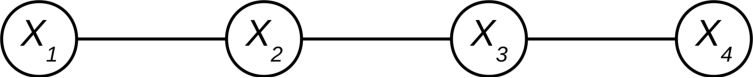
\includegraphics[width=0.4\columnwidth]{./figs/17_2_a.pdf}
      \label{fig:chap_17_2_a}
    \end{figure}
  \end{exerciseSection}
  
  \begin{exerciseSection}
    Same as (a).
  \end{exerciseSection}
  
  \begin{exerciseSection}
    \begin{figure}[htb]
      \centering
      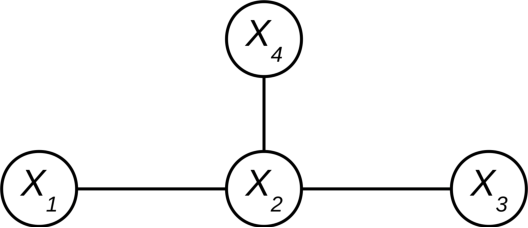
\includegraphics[width=0.3\columnwidth]{./figs/17_2_c.pdf}
      \label{fig:chap_17_2_c}
    \end{figure}
  \end{exerciseSection}
\end{exercise}

\begin{exercise}
  \begin{exerciseSection}
    Since
    \begin{align}
      \left[
        \begin{array}{cc}
          \mathbf{\Theta}_{aa} & \mathbf{\Theta}_{ab} \\
          \mathbf{\Theta}_{ba} & \mathbf{\Theta}_{bb}
        \end{array}
      \right]
      \left[
        \begin{array}{cc}
          \mathbf{\Sigma}_{aa} & \mathbf{\Sigma}_{ab} \\
          \mathbf{\Sigma}_{ba} & \mathbf{\Sigma}_{bb}
        \end{array}
      \right] = \mathbf{I}
    \end{align}
    therefore we have
    \begin{subequations}
      \begin{align}
        \mathbf{\Theta}_{aa}\mathbf{\Sigma}_{aa} +
        \mathbf{\Theta}_{ab}\mathbf{\Sigma}_{ba} = \mathbf{I}
        \label{eq:chap_17_3_a_1}
        \\
        \mathbf{\Theta}_{aa}\mathbf{\Sigma}_{ab} +
        \mathbf{\Theta}_{ab}\mathbf{\Sigma}_{bb} = \mathbf{0}
        \label{eq:chap_17_3_a_2}
      \end{align}
    \end{subequations}
    \eqref{eq:chap_17_3_a_1} -
    \eqref{eq:chap_17_3_a_2}$\mathbf{\Sigma}_{bb}^{-1}\mathbf{\Sigma}_{ba}$, we
    have
    \begin{align}
      \mathbf{\Theta}_{aa}\left(\mathbf{\Sigma}_{aa} -
      \mathbf{\Sigma}_{ab} \mathbf{\Sigma}_{bb}^{-1}\mathbf{\Sigma}_{ba} \right)
      = \mathbf{I}
    \end{align}
    consequently $\mathbf{\Theta}_{aa}^{-1} = \mathbf{\Sigma}_{a, b}$.
  \end{exerciseSection}
  
  \begin{exerciseSection}
    Assume that $\Sigma_{12} = 0$, i.e. $\mathbf{\Sigma}_{aa}$ is diagonal. From
    (a) $\mathbf{\Sigma}_{a, b}$ is also diaonal, which suggests that
    $\mbox{cov}(X_1, X_2|\mbox{rest}) = 0$.
  \end{exerciseSection}
  
  \begin{exerciseSection}
    Since $r_{jk} = \Theta_{jk} / \sqrt{\Theta_{jj} \Theta_{kk}}$, for $j=k$, we
    have $r_{jk} = 1$. For $j\not=k$, denote $X_a = (X_k, X_k)$, then
    \begin{align}
      \left[
        \begin{array}{cc}
          \Theta_{jj} & \Theta_{jk} \\ 
          \Theta_{kj} & \Theta_{kk}
        \end{array}
      \right] = \mathbf{\Theta}_{aa} =
      \left[
        \begin{array}{cc}
          \Sigma_{jj|\mbox{rest}} & \Sigma_{jk|\mbox{rest}} \\ 
          \Sigma_{kj|\mbox{rest}} & \Sigma_{kk|\mbox{rest}}
        \end{array}
      \right]^{-1}
    \end{align}
    therefore
    \begin{subequations}
      \begin{align}
        \Theta_{jj} \Sigma_{jj|\mbox{rest}} + \Theta_{jk}
        \Sigma_{kj|\mbox{rest}} &= 1 \\
        \Theta_{jj} \Sigma_{jk|\mbox{rest}} + \Theta_{jk}
        \Sigma_{kk|\mbox{rest}} &= 0 \\
        \Theta_{kj} \Sigma_{jk|\mbox{rest}} + \Theta_{kk}
        \Sigma_{kk|\mbox{rest}} & = 1
      \end{align}
    \end{subequations}
    consequently, we have
    \begin{subequations}
      \begin{align}
        \Theta_{jj} \Sigma_{jj|\mbox{rest}} & = \Theta_{kk}
        \Sigma_{kk|\mbox{rest}} \\
        \Theta_{jk} \Sigma_{kk|\mbox{rest}} & = \Theta_{jj}
        \Sigma_{jk|\mbox{rest}}
      \end{align}
    \end{subequations}
    As a result, $r_jk = -\Sigma_{jk|\mbox{rest}} /
    \sqrt{\Sigma_{jj|\mbox{rest}} \Sigma_{kk|\mbox{rest}}} =
    -\rho_{jk|\mbox{rest}}$.
  \end{exerciseSection}
\end{exercise}

\begin{exercise}
  Since
  \begin{align}
    f(X_1|X_2, \mbox{rest}) = \frac{f(X_1, X_2| \mbox{rest})}{f(X_2|
    \mbox{rest})} = f(X_1|\mbox{rest})
  \end{align}
  we have
  \begin{align}
    f(X_1, X_2| \mbox{rest}) = f(X_1|\mbox{rest}) f(X_2|\mbox{rest})
  \end{align}
  i.e. $X_1\perp X_2|\mbox{rest}$.
\end{exercise}

\begin{exercise}
  Since there is no missing edges
  \begin{align}
    l_C(\mathbf{\Theta}) = l(\mathbf{\Theta}) = \log|\mathbf{\Theta}| -
    \tr(\mathbf{S\Theta})
  \end{align}
  The gradient equation for maximizing $l_C(\mathbf{\Theta})$ becomes
  $\mathbf{\Theta}^{-1} - \mathbf{S} = 0$, which suggests
  \begin{align}
    \mathbf{S\Theta} = 
    \left[
      \begin{array}{cc}
        \mathbf{S}_{11} & \mathbf{s}_{12} \\
        \mathbf{s}_{12}^T & s_{22}
      \end{array}
    \right]
    \left[
      \begin{array}{cc}
        \mathbf{\Theta}_{11} & \bm{\theta}_{12} \\
         \bm{\theta}_{12}^T & \theta_{22}
      \end{array}
    \right] = 
    \left[
      \begin{array}{cc}
        \mathbf{I} & \mathbf{0} \\
         \mathbf{0}^T & 1
      \end{array}
    \right] 
  \end{align}
  therefore
  \begin{align}
    \mathbf{S}_{11}\bm{\theta}_{12} + \theta_{22}\mathbf{s}_{12} = 0
  \end{align}
  Since $\bm{\beta} = -\bm{\theta}_{12} / \theta_{22}$ as in (17.9), we have
  $\mathbf{S}_{11}\bm{\beta} - \mathbf{s}_{12} = 0$.
\end{exercise}

\begin{exercise}
  Since 
  \begin{align}
    \left[
      \begin{array}{cc}
        \mathbf{W}_{11} & \mathbf{w}_{12} \\
        \mathbf{w}_{12}^T & w_{22}
      \end{array}
    \right]
    \left[
      \begin{array}{cc}
        \mathbf{\Theta}_{11} & \bm{\theta}_{12} \\
         \bm{\theta}_{12}^T & \theta_{22}
      \end{array}
    \right] = 
    \left[
      \begin{array}{cc}
        \mathbf{I} & \mathbf{0} \\
         \mathbf{0}^T & 1
      \end{array}
    \right] 
  \end{align}
  we have
  \begin{subequations}
    \begin{align}
      \mathbf{W}_{11}\bm{\theta}_{12} + \theta_{22}\mathbf{w}_{12} & = 0 \\
      \mathbf{w}_{12}^T\bm{\theta}_{12} + \theta_{22}w_{22} & = 1
    \end{align}
  \end{subequations}
  therefore
  \begin{subequations}
    \begin{align}
      \bm{\theta}_{12} &= -\mathbf{W}_{11}^{-1}\mathbf{w}_{12}\theta_{22} =
      -\hat{\bm{\beta}}\theta_{22} \\
      \theta_{22} &= \frac{1 - \mathbf{w}_{12}^T\bm{\theta}_{12}}{w_{22}}
    \end{align}
  \end{subequations}
  Combining these 2 equations, we have
  \begin{align}
    \theta_{22} = \frac{1}{w_22 -
    \mathbf{w}_{12}^T\mathbf{W}_{11}^{-1}\mathbf{w}_{12}}
  \end{align}
\end{exercise}

\begin{exercise}[(Program)]
\end{exercise}

\begin{exercise}[(Program)]
\end{exercise}

\begin{exercise}
  \begin{exerciseSection}
    \emph{E-step:} The missing data (latent variables), given the current
    estimation $\hat{\bm{\mu}}$, $\hat{\mathbf{\Sigma}}$ and the observed data,
    follow Gaussian distribution as
    \begin{align}
      \mathbf{x}_{i, m_i}\sim\mathcal{N}\left(\hat{\bm{\mu}}_{m_i} +
     \hat{\mathbf{\Sigma}}_{m_i, o_i} \hat{\mathbf{\Sigma}}_{o_i,
      o_i}^{-1} (\mathbf{x}_{i, o_i} - \hat{\bm{\mu}}_{o_i}),
      \hat{\mathbf{\Sigma}}_{m_i, m_i} - \hat{\mathbf{\Sigma}}_{m_i, o_i}
      \hat{\mathbf{\Sigma}}_{o_i, o_i}^{-1} \hat{\mathbf{\Sigma}}_{o_i, m_i}
      \right)
    \end{align}
    (here $\mathbf{x}_{i, m_i}$, $\mathbf{x}_{i, o_i}$ and
    $\hat{\bm{\mu}}_{m_i}$, $\hat{\bm{\mu}}_{o_i})$ are written as column
    vectors.) Therefore, the expectation of the log-likelihood of the data
    over the above conditional distribtion of $\mathbf{x}_{i, m_i}$ is
    \begin{align}
      \mathbb{E}\left[l(\bm{\mu}, \mathbf{\Sigma}; \mathbf{X}_o,
      \mathbf{X}_m)\right] & = C+ N\log|\mathbf{\Sigma}^{-1}| -
      \tr\left(\mathbb{E}\left[(\mathbf{X} - \mathbf{1}\bm{\mu}^T)
      \mathbf{\Theta} (\mathbf{X} - \mathbf{1}\bm{\mu}^T)^T \right] \right)
      \notag
      \\
      &=  C+ N\log|\mathbf{\Sigma}^{-1}|-
      \sum_{i=1}^N
      \sum_{j=1}^p \sum_{k=1}^p\mathbb{E}\left[(x_{ij} - \mu_j)\Theta_{jk}
      (x_{ik} - \mu_k) \right]
    \end{align}
    where $\mathbf{\Theta} = \mathbf{\Sigma}^{-1}$
        
    \emph{M-step: } To maximize the log likelihood, we have
    \begin{align}
      \pdv{\mathbb{E}\left[l(\bm{\mu}, \mathbf{\Sigma}; \mathbf{X}_o,
      \mathbf{X}_m)\right]}{\bm{\mu}} &= \mathbf{1}^T\mathbb{E}[\mathbf{X} -
      \mathbf{1}\bm{\mu}^T]\mathbf{\Theta} = \mathbf{0}
    \end{align}
    thus $\hat{\bm{\mu}} = \mathbb{E}[\mathbf{X}^T\mathbf{1}] / N =
    \hat{\mathbf{X}}^T\mathbf{1} / N$, where $\hat{\mathbf{X}}$ represents the
    $N$-by-$p$ predictor matrix with the missing entries replaced by the imputed
    ones, namely the mean of $\mathbf{x}_{i, m_i}$. Also we have
    \begin{align}
      \pdv{\mathbb{E}\left[l(\bm{\mu}, \mathbf{\Sigma}; \mathbf{X}_o,
      \mathbf{X}_m)\right]}{\mathbf{\Theta}} &= N\mathbf{\Sigma} -
      \mathbb{E} \left[(\mathbf{X} - \mathbf{1}\bm{\mu}^T)^T(\mathbf{X} -
      \mathbf{1}\bm{\mu}^T) \right] = \mathbf{0}
    \end{align}
    therefore, the ML estimation of $\mathbf{\Sigma}$ is
    \begin{align}
      \hat{\mathbf{\Sigma}} = \frac{1}{N} \mathbb{E} \left[(\mathbf{X} -
      \mathbf{1}\hat{\bm{\mu}}^T)^T(\mathbf{X} - \mathbf{1}\hat{\bm{\mu}}^T)
      \right]
    \end{align}
    Denote $E_{ijk} = \mathbb{E}\left[(x_{ij} - \hat{\mu}_j)(x_{ik} -
    \hat{\mu}_k) \right]$, since
    \begin{align}
      E_{ijk} &= (\mathbb{E}[x_{ij}] - \hat{\mu}_j)(\mathbb{E}[x_{ik}] -
      \hat{\mu}_k) + \mbox{cov}(x_{ij}x_{ik})
    \end{align}
    in which 
    \begin{align}
      \mathbb{E}[x_{ij}] = \hat{x}_{ij},\;\mathbb{E}[x_{ik}] = \hat{x}_{ik}
    \end{align}
    whether $j,k\in m_i$ or not, and
    \begin{align}
      \mbox{cov}(x_{ij}x_{ik}) = \left\{
        \begin{array}{ll}
          0 & \mbox{if } j\in o_i \mbox{ or } k\in o_i \\
          \hat{\Sigma}_{jk} & \mbox{otherwise}
        \end{array}
      \right.
    \end{align}
    therefore (17.44) is proved, in which the correction term $c_{i, jj'}$
    corresponds to the the non-zero covariance $\mbox{cov}(x_{ij}x_{ij'})$ when
    both $j$ and $j'$ are imputed for $x_i$.
  \end{exerciseSection}
  
  \begin{exerciseSection}
    (Program)
  \end{exerciseSection}
  
  \begin{exerciseSection}
    (Program)
  \end{exerciseSection}
\end{exercise}

\begin{exercise}
  An absence of the constant node $X_0 \equiv 1$ ill lead to the following
  ambiguity
  \begin{align}
    p(X_1=0, X_2=0) = p(X_1=1, X_2=0) = p(X_1=0, X_2=1)
  \end{align}
  only by including $X_0 \equiv 1$ the 4 possible values can be uniquely
  defined. \begin{figure}[htb]
      \centering
      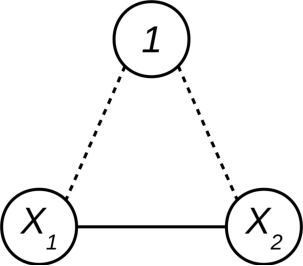
\includegraphics[width=0.15\columnwidth]{./figs/17_10.pdf}
      \label{fig:chap_17_10}
    \end{figure}
\end{exercise}

\begin{exercise}
  \begin{align}
    p(X_j=1|X_{\mbox{rest}} = x_{\mbox{rest}}, \mathbf{\Theta}) &=
    \frac{p(X_j=1,X_{\mbox{rest}} = x_{\mbox{rest}} |
    \mathbf{\Theta})}{p(X_{\mbox{rest}} = x_{\mbox{rest}} | \mathbf{\Theta})}
    \notag \\
    &= \frac{p(X_j=1,X_{\mbox{rest}} = x_{\mbox{rest}} |
    \mathbf{\Theta})} {p(X_j=1, X_{\mbox{rest}} = x_{\mbox{rest}} |
    \mathbf{\Theta}) + p(X_j=0, X_{\mbox{rest}} = x_{\mbox{rest}} |
    \mathbf{\Theta})} \notag \\
    &= \frac{C\exp\left(\sum_{k:(j,k)\in
    E}\theta_{jk}x_k\right)}{C\exp\left(\sum_{k:(j,k)\in E}\theta_{jk}x_k\right)
    + C} \notag \\
    &= \frac{1} 
    {1 + \exp\left(-\sum_{k:(j,k)\in E}\theta_{jk}x_k\right)}
  \end{align}
  where $C$ is a constant given the value of the rest nodes in the graph. Now
  this probability has the logistic form as (17.30) (considering a
  constant node $X_0=1$).
\end{exercise}

\begin{exercise}
  ???
\end{exercise} % Chapter 17
\chapter{High-Dimensional Problems}
\label{ch:18} % Chapter 18

\appendix
\newpage

\bibliographystyle{IEEEtran}
\bibliography{refs.bib}


\end{document}
